\documentclass[12pt,a4paper]{article}

% ===================== PACOTES (mesmo estilo dos relatórios de Lab. de Biologia Molecular) =====================
\usepackage[utf8]{inputenc}
\usepackage[T1]{fontenc}
\usepackage[brazilian]{babel}
\usepackage[a4paper,left=3cm,right=2cm,top=3cm,bottom=2cm]{geometry}
\usepackage{times}
\usepackage{setspace}
\usepackage{indentfirst}
\usepackage{graphicx}
\usepackage{booktabs}
\usepackage{array}
\usepackage{xcolor}
\usepackage{float}
\usepackage{textcomp}
\usepackage[font=footnotesize,labelfont=bf,labelsep=period,skip=4pt]{caption}
\usepackage{hyperref}

\hypersetup{
  colorlinks=true,
  linkcolor=black,
  citecolor=black,
  urlcolor=blue,
  pdftitle={Rede de interação do gene HTT na Doença de Huntington: hubs, robustez e cascata de falha},
  pdfauthor={Vinícius Massaru Oliveira Tanaka; Marcos Vinícius Magalhães Alves}
}

\graphicspath{{imagens/}}

\setstretch{1.06}
\setlength{\parindent}{1.25cm}
\setlength{\parskip}{0pt}
% evita que citações longas, como [BULDYREV et al., 2010], ultrapassem a margem
\sloppy
\setlength{\emergencystretch}{3em}

\renewcommand{\figurename}{Figura}
\renewcommand{\tablename}{Tabela}
\renewcommand{\refname}{Referências}

% Marcador amarelo para o que o autor precisa conferir ou preencher
% (apague o macro e deixe só o texto quando terminar a revisão)
\newcommand{\conf}[1]{\colorbox{yellow}{\textbf{[#1]}}}
% linha de fonte das figuras, em corpo menor que a legenda
\newcommand{\fonte}[1]{\par\vspace{2pt}{\footnotesize Fonte: #1}}

\newif\ifcapa
\capatrue

\begin{document}

\ifcapa
\begin{titlepage}
  \begin{center}
    \Large
    Universidade Federal de São Paulo\\
    Instituto de Ciência e Tecnologia
    \vspace*{1cm}

    
\includegraphics[width=6cm]{Unifesp_completa_policromia_RGB.png}\\
    \vspace*{3cm}

    \huge
    \textbf{Rede de interação do gene HTT na Doença de Huntington: hubs, robustez e cascata de falha}\\
    \vspace*{1cm}
    \Large
    Introdução à Biologia de Sistemas
  \end{center}
  \vspace*{1.5cm}
  \begin{flushright}
    \Large
    \textbf{Alunos:}\\
    \large
    Vinícius Massaru Oliveira Tanaka\\
    Marcos Vinícius Magalhães Alves\\[0.5cm]
    \textbf{Professor:} André Zelanis
  \end{flushright}
  \vspace*{\fill}
  \begin{center}\large São José dos Campos\\ 2026\end{center}
\end{titlepage}
\fi

% ===================== 1. INTRODUÇÃO =====================
\section{Introdução}

A Doença de Huntington (DH) é uma doença neurodegenerativa hereditária causada por uma expansão de repetições do trinucleotídeo CAG no gene \textit{HTT}, localizado no cromossomo 4 \cite{htt1993}. Alelos com até 26 repetições são normais, de 27 a 35 são intermediários, de 36 a 39 têm penetrância reduzida e, a partir de 40 repetições, a doença se manifesta com certeza ao longo da vida \cite{genereviews} (Figura~\ref{fig:cag}). Os sinais incluem movimentos involuntários (coreia), rigidez muscular, alterações da marcha, dificuldades de fala e deglutição e alterações cognitivas e emocionais, com início geralmente na vida adulta \cite{genereviews}. A prevalência estimada é de cerca de 4,9 casos por 100\,000 habitantes, e é maior na Europa e na América do Norte \cite{medina2022}.

Como a huntingtina participa de vários processos celulares ao mesmo tempo, a DH é um bom exemplo para a biologia de sistemas: em vez de um único gene, estudamos a rede de proteínas em torno dele \cite{barabasi2004}. A expansão CAG produz uma huntingtina com região de poliglutamina aumentada, associada a um ganho de função tóxico, mas a huntingtina normal também participa de processos celulares relevantes. Por isso é importante distinguir reduzir a toxicidade de eliminar a proteína. O trabalho tem três objetivos: (i) montar e caracterizar a rede de interação proteína-proteína (PPI) do HTT; (ii) identificar seus hubs e pontes; (iii) testar a robustez da rede à remoção de nós e simular a propagação de falhas, para sugerir quais proteínas merecem atenção como alvos de investigação. A rede foi construída por curadoria de processos biológicos e pela integração de associações já existentes no STRING, e não pela descoberta experimental de novas interações.

\begin{figure}[H]
  \centering
  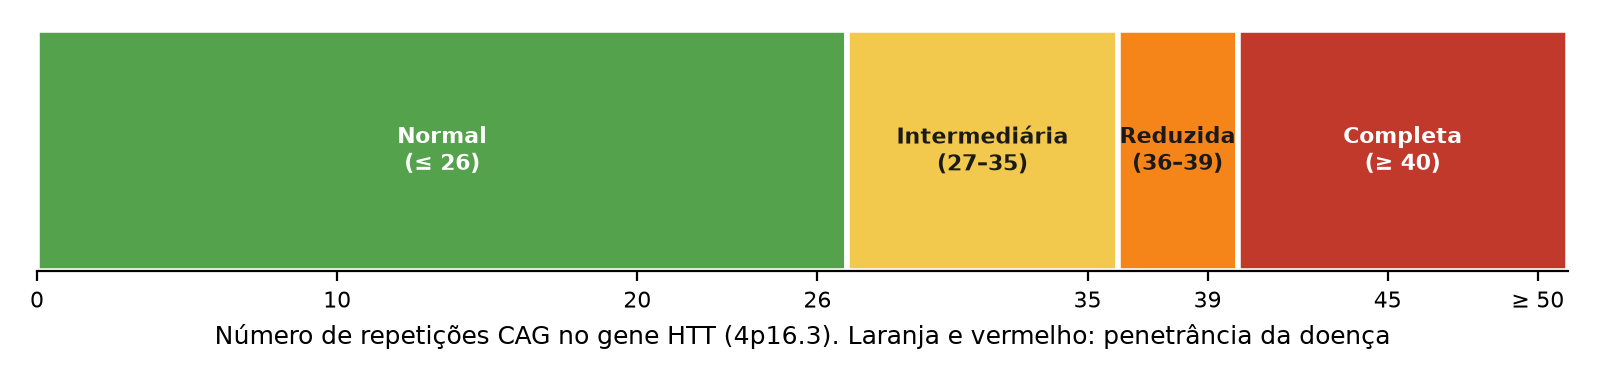
\includegraphics[width=0.95\textwidth]{fig_cag.png}
  \caption{Faixas de repetições CAG no gene \textit{HTT} e penetrância da doença.}
  \label{fig:cag}
  \fonte{Elaborada pelos autores, com base em \cite{genereviews}.}
\end{figure}

% ===================== 2. MÉTODOS =====================
\section{Materiais e métodos}

\textbf{Obtenção dos dados.} Partimos do mapa da Doença de Huntington do KEGG \cite{kegg2000,keggpath} (Apêndice~A) e da literatura, que orientaram a seleção de 33 proteínas iniciais, distribuídas em sete grupos funcionais definidos biologicamente antes da análise: transporte intracelular, transcrição, sinalização de cálcio, mitocôndria e estresse oxidativo, apoptose, autofagia e função astrocitária. Cada grupo foi consultado separadamente no STRING \cite{string2025,stringsite}, sem o HTT, com expansão de uma camada de interações. Os resultados somaram 67 proteínas, e o HTT, que não retornou nas consultas, foi acrescentado manualmente na consulta integrada, totalizando 68 nós e 367 associações. O STRING atribui a cada associação uma pontuação de confiança de 0 a 1. No Cytoscape, mantivemos as arestas com pontuação $\geq 0{,}7$ (alta confiança) e os nós ligados a elas, o que resultou em 66 nós e 207 arestas (consultas ao KEGG e ao STRING, versão 12.5, realizadas em 13 e 14 de novembro de 2026). Os nós representam proteínas, identificadas por símbolos gênicos, e as arestas representam associações funcionais, que incluem interação física e participação em uma mesma via. A pontuação indica confiança, e não a intensidade de uma ligação física. A rede é não direcionada e as interações não têm sinal.

\textbf{Análise topológica.} A rede foi importada no Cytoscape 3.10.5 \cite{shannon2003} e analisada com o NetworkAnalyzer (grau, densidade, coeficiente de agrupamento, caminho médio, diâmetro, heterogeneidade, centralização e betweenness). Os mesmos valores foram reproduzidos em Python (biblioteca \textit{networkx}) como conferência. As posições dos nós nas figuras vêm do layout de forças do Cytoscape.

\textbf{Mundo pequeno.} Comparamos o coeficiente de agrupamento $C$ e o caminho médio $L$ da rede com os de 300 redes aleatórias de Erdős--Rényi (mesmo número de nós e de arestas) e de 300 redes geradas pelo modelo de configuração (mesma sequência de graus). Calculamos $\sigma = (C/C_r)/(L/L_r)$, em que $C_r$ e $L_r$ são as médias das redes aleatórias; $\sigma > 1$ indica propriedade de mundo pequeno. Também ajustamos uma lei de potência à distribuição de graus para avaliar se a rede poderia ser livre de escala.

\textbf{Modularidade.} Medimos a modularidade $Q$ \cite{newman2006} da partição nos sete grupos funcionais e a comparamos com a partição encontrada de forma independente pelo algoritmo de Louvain \cite{blondel2008}.

\textbf{Robustez.} Removemos até 25 nós (38\% da rede) de três formas: ao acaso (média de 200 sorteios), por ataque ao maior grau e por ataque à maior betweenness, recalculando a métrica depois de cada remoção, como em \cite{albert2000}. Medimos a fração do maior componente conexo e a eficiência global (média do inverso das distâncias entre pares de nós). Também removemos cada nó individualmente e identificamos os pontos de articulação, isto é, os nós cuja remoção desconecta a rede.

\textbf{Cascata de falha.} Simulamos a propagação de falhas por limiar, no espírito de \cite{buldyrev2010}: um nó falha quando a fração de seus vizinhos já falhos é de pelo menos $\varphi$. Iniciamos a cascata a partir de cada nó e testamos $\varphi = 0{,}2;\ 0{,}3;\ 0{,}4;\ 0{,}5$. O valor de $\varphi$ é uma suposição nossa e por isso foram testados vários. 

\textbf{Estratégia de proteção.} Para propor uma solução, invertemos a pergunta: quais proteínas, se protegidas (impedidas de falhar), mais contêm a cascata? Comparamos quatro formas de escolher $k = 1$ a 5 proteínas: ao acaso (média de 40 sorteios), pelos maiores graus, pelas maiores betweenness e por escolha gulosa, em que a cada passo se adiciona a proteína que mais reduz o tamanho médio da cascata. O critério é o número médio de nós que falham, partindo de cada nó como semente.

Os \textit{scripts}, os dados e uma versão interativa da rede estão em \url{https://github.com/vimassaru/huntington-rede}.

% ===================== 3. RESULTADOS =====================
\section{Resultados}

\subsection{Características da rede}

A rede final (Figura~\ref{fig:rede}) tem 66 nós e 207 arestas, é conexa e apresenta grau médio de 6,27, densidade de 0,097, coeficiente de agrupamento de 0,64, caminho médio de 2,95, diâmetro 6 e raio 3 (Tabela~\ref{tab:metricas}). Apenas 9,7\% das conexões possíveis estão presentes, ou seja, a rede é esparsa. O coeficiente de agrupamento alto e o caminho médio curto indicam uma rede densamente agrupada e com proteínas separadas por poucas conexões. A distribuição de graus (Figura~\ref{fig:grau}a) tem pico entre 5 e 6 conexões e cauda curta, sem seguir uma lei de potência clara. Com 66 nós, isso não permite afirmar que a rede seja livre de escala.

\begin{table}[H]
  \centering
  \caption{Características globais da rede PPI do HTT (STRING, pontuação $\geq$ 0,7).}
  \label{tab:metricas}
  \footnotesize
  \begin{tabular}{lr@{\hspace{1.2cm}}lr}
    \toprule
    Nós & 66 & Coef. de agrupamento & 0,64 \\
    Arestas & 207 & Caminho médio & 2,95 \\
    Grau médio & 6,27 & Diâmetro / raio & 6 / 3 \\
    Densidade & 0,097 & Componentes conexos & 1 \\
    Heterogeneidade & 0,617 & Centralização & 0,186 \\
    \bottomrule
  \end{tabular}
\end{table}

\begin{figure}[H]
  \centering
  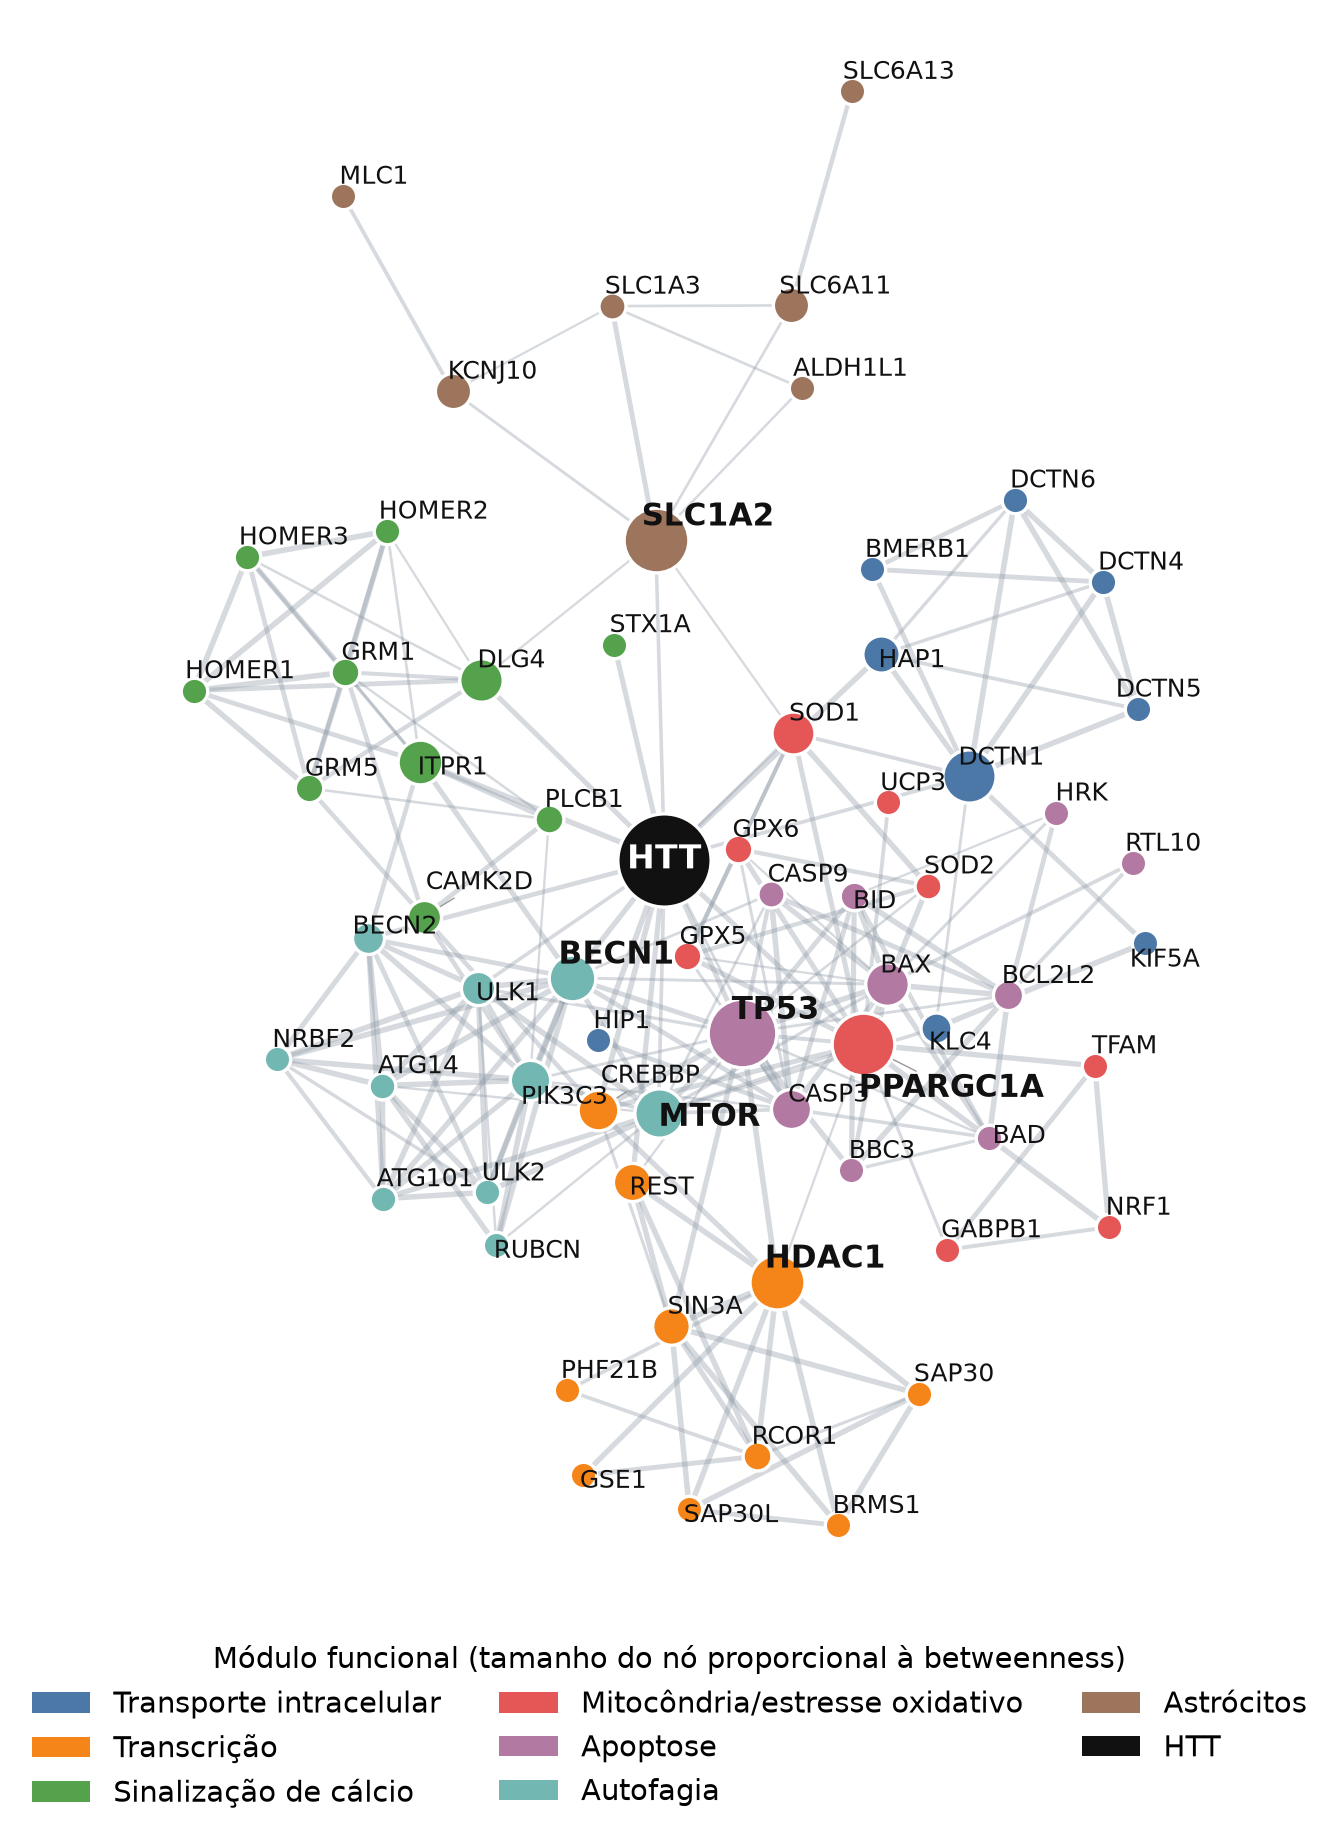
\includegraphics[width=\textwidth,height=0.8\textheight,keepaspectratio]{rede_modulos.png}
  \caption{Rede PPI do HTT. A cor indica o módulo funcional e o tamanho do nó é proporcional à betweenness. O HTT (preto) ocupa o centro e liga os módulos.}
  \label{fig:rede}
  \fonte{Elaborada pelos autores, com dados do STRING \cite{string2025}. Layout calculado no Cytoscape 3.10.5 \cite{shannon2003}.}
\end{figure}

\subsection{Mundo pequeno}

O coeficiente de agrupamento da rede (0,64) é de 5 a 7 vezes maior que o de redes aleatórias do mesmo tamanho (0,09 em Erdős--Rényi e 0,12 com os mesmos graus), enquanto o caminho médio é parecido (2,95 contra 2,45 e 2,57; Figura~\ref{fig:sw}). Isso dá $\sigma = 5{,}6$ em relação às redes de Erdős--Rényi e $\sigma = 4{,}7$ em relação ao modelo de configuração, ambos bem acima de 1: a rede tem a propriedade de mundo pequeno. Já a distribuição de graus é heterogênea, mas o ajuste de uma lei de potência foi instável (expoente entre 1,4 e 2,1, conforme o grau mínimo considerado), de modo que não afirmamos que a rede seja livre de escala.

\begin{figure}[H]
  \centering
  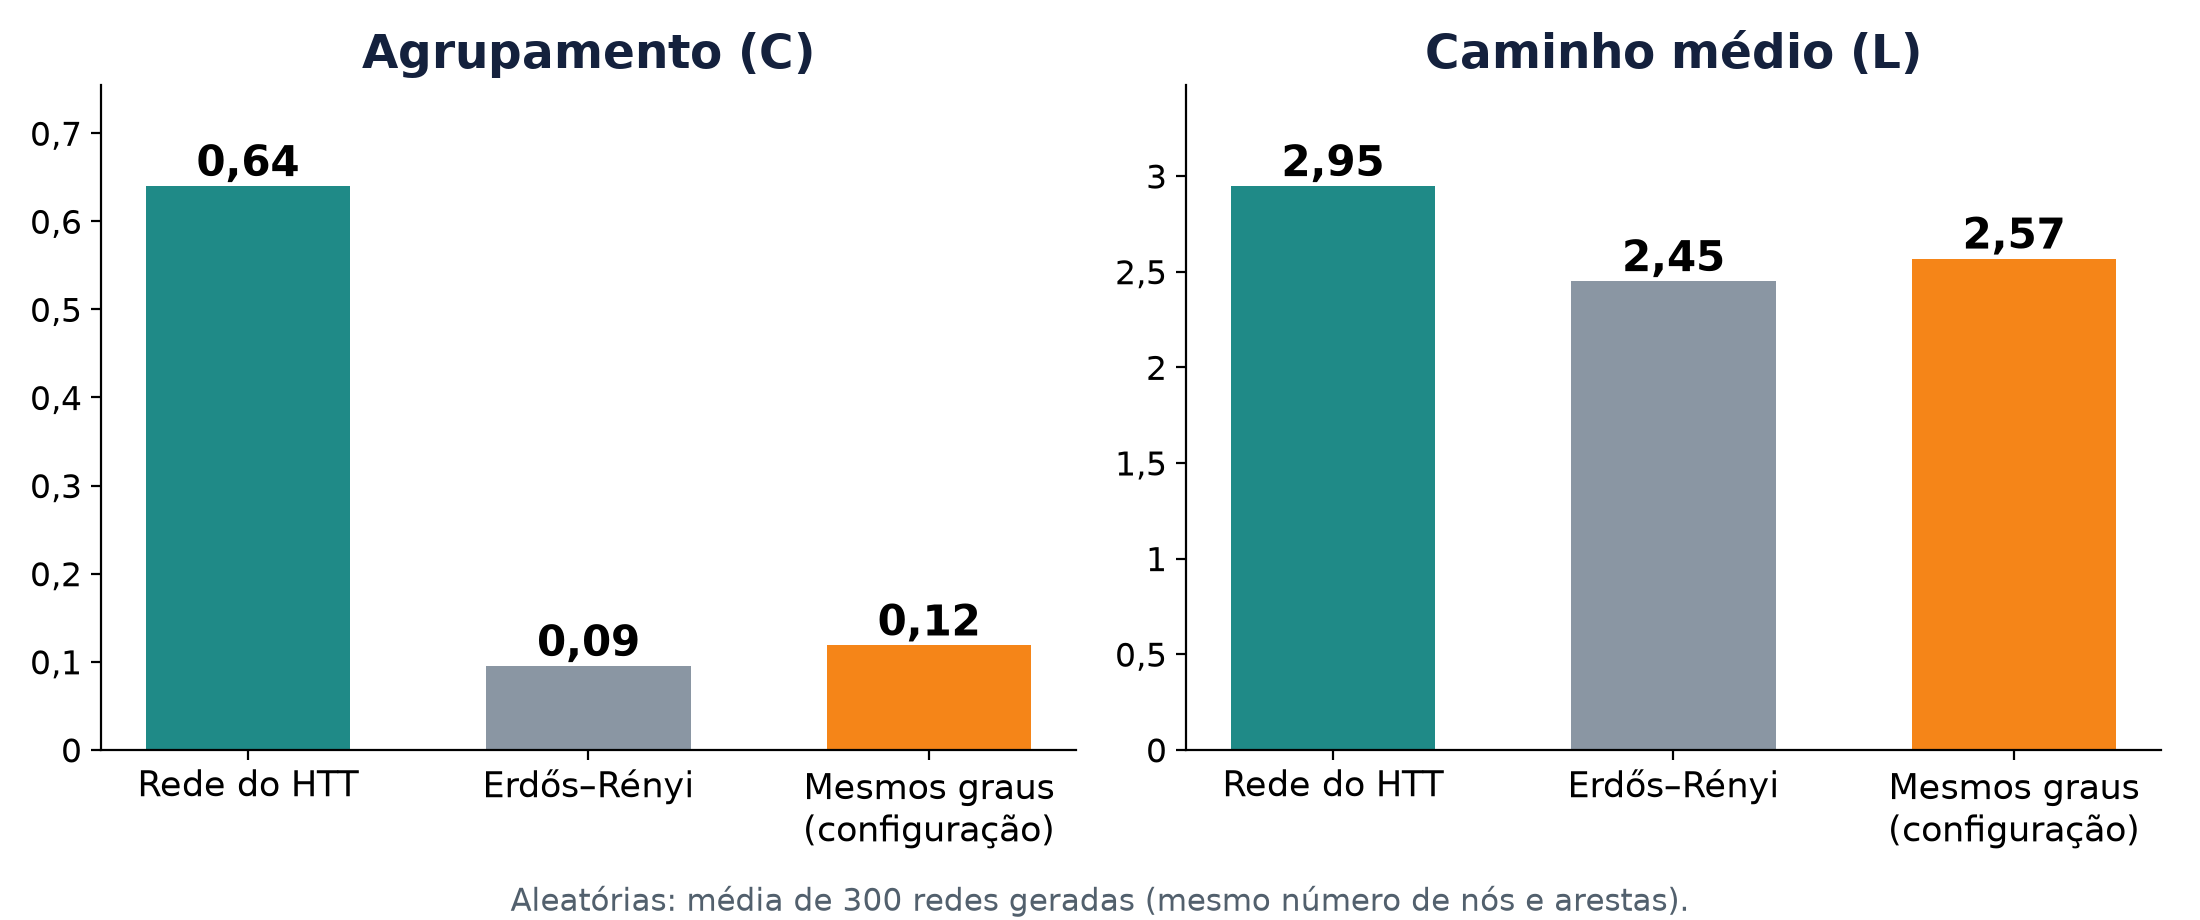
\includegraphics[width=0.95\textwidth]{fig_smallworld.png}
  \caption{Coeficiente de agrupamento e caminho médio da rede do HTT e de redes aleatórias (média de 300 redes de cada tipo).}
  \label{fig:sw}
  \fonte{Elaborada pelos autores (Python, \textit{networkx}).}
\end{figure}

\subsection{Módulos funcionais e modularidade}

Os sete grupos funcionais definidos a partir do KEGG se comportam como comunidades da rede (Tabela~\ref{tab:modulos}). Dentro dos módulos ficam 156 das 207 arestas (75\%), e a modularidade da partição funcional é $Q = 0{,}60$. O algoritmo de Louvain, que não conhece a função das proteínas, encontra 7 comunidades com $Q = 0{,}61$. Ou seja, a organização funcional descrita na literatura aparece na topologia da rede. Os módulos de apoptose e autofagia têm mais conexões para fora (24 e 21) e são os mais ligados ao resto, enquanto o módulo astrocitário é o mais isolado (3 arestas para fora, além da ligação com o HTT).

\begin{table}[H]
  \centering
  \caption{Módulos funcionais da rede: número de nós, grau médio, arestas dentro e para fora do módulo e proteínas de maior grau.}
  \label{tab:modulos}
  \footnotesize
  \begin{tabular}{p{3.6cm}rrrrp{3.6cm}}
    \toprule
    Módulo & Nós & Grau médio & Arestas internas & Arestas externas & Principais proteínas \\
    \midrule
    Transporte intracelular & 9 & 4,2 & 16 & 6 & DCTN1, DCTN6, HAP1 \\
    Transcrição & 10 & 5,3 & 22 & 9 & HDAC1, SIN3A, CREBBP \\
    Sinalização de cálcio & 10 & 5,9 & 25 & 9 & GRM1, ITPR1, GRM5 \\
    Mitocôndria e estresse oxidativo & 9 & 5,2 & 17 & 13 & PPARGC1A, SOD1, GPX5 \\
    Apoptose & 10 & 8,0 & 28 & 24 & TP53, BAX, CASP3 \\
    Autofagia & 10 & 9,9 & 39 & 21 & BECN1, MTOR, PIK3C3 \\
    Astrócitos & 7 & 3,0 & 9 & 3 & SLC1A2, SLC1A3, SLC6A11 \\
    HTT & 1 & 17,0 & 0 & 17 & HTT \\
    \bottomrule
  \end{tabular}
\end{table}

\subsection{Hubs e pontes}

O TP53 é o nó com mais conexões (grau 18), seguido do HTT (17), do BECN1 (15) e do MTOR (14). A betweenness destaca outro conjunto: o HTT tem o maior valor (0,399), cerca do dobro do TP53 (0,200), e o SLC1A2, do módulo astrocitário, aparece em terceiro (0,174), mesmo com apenas sete conexões (Figura~\ref{fig:grau}b e Tabela~\ref{tab:hubs}). O TP53 se destaca pela quantidade de associações diretas, enquanto o HTT, o SLC1A2 e o PPARGC1A funcionam como pontes entre os módulos.

\begin{figure}[H]
  \centering
  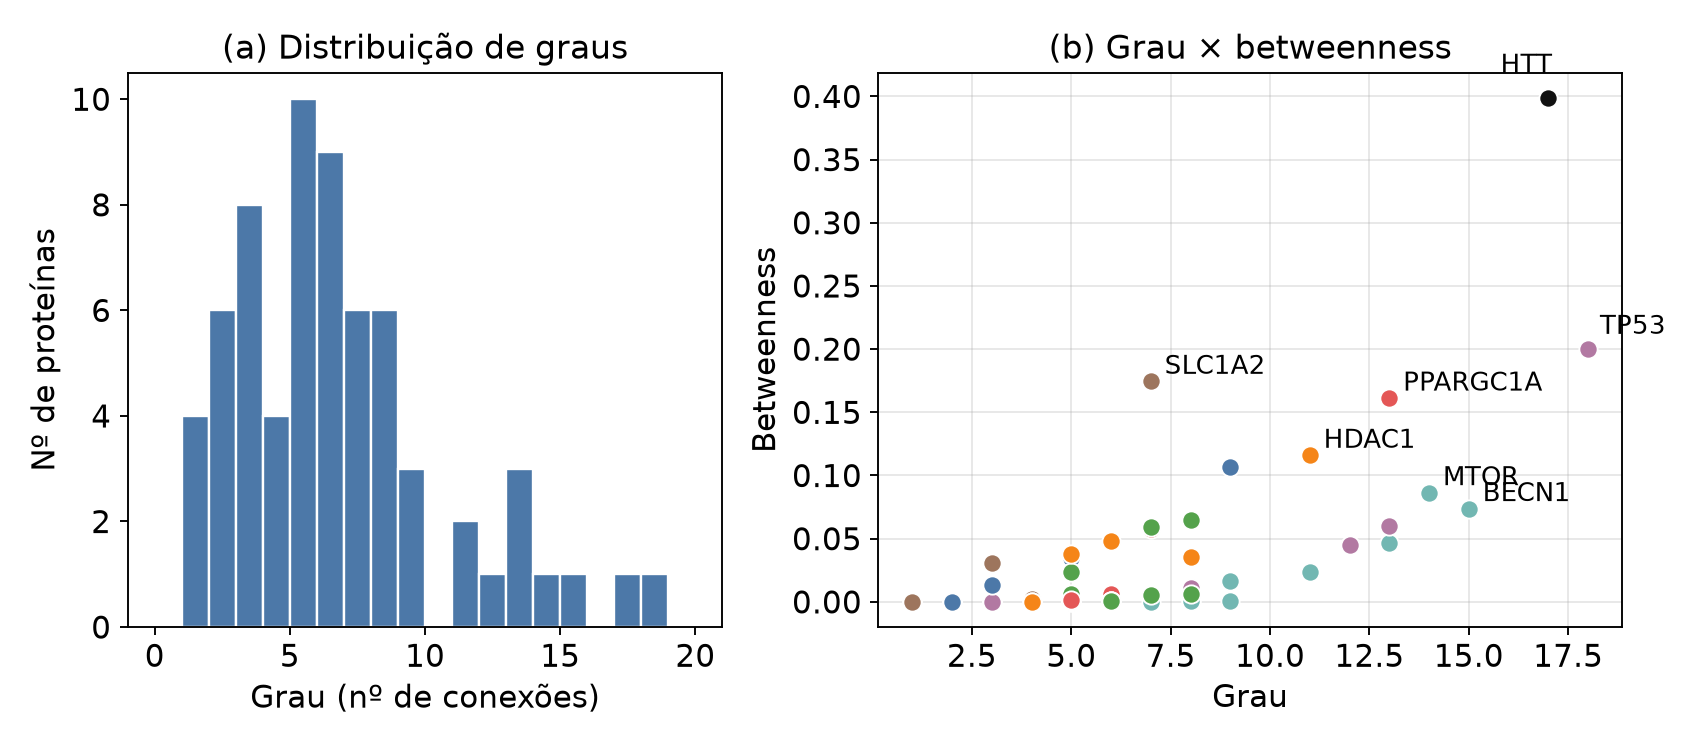
\includegraphics[width=\textwidth]{fig_grau.png}
  \caption{(a) Distribuição de graus. (b) Grau e betweenness de cada proteína, coloridas por módulo. As proteínas de alta betweenness e grau baixo ou médio (SLC1A2, PPARGC1A) são pontes.}
  \label{fig:grau}
  \fonte{Elaborada pelos autores.}
\end{figure}

\begin{table}[H]
  \centering
  \caption{Nós de maior grau e de maior betweenness.}
  \label{tab:hubs}
  \footnotesize
  \begin{tabular}{llrr}
    \toprule
    Proteína & Módulo & Grau & Betweenness \\
    \midrule
    TP53 & Apoptose & 18 & 0,200 \\
    HTT & Proteína central & 17 & 0,399 \\
    SLC1A2 & Astrócitos & 7 & 0,174 \\
    PPARGC1A & Mitocôndria/estresse oxidativo & 13 & 0,161 \\
    HDAC1 & Transcrição & 11 & 0,116 \\
    \bottomrule
  \end{tabular}
\end{table}

\subsection{Robustez à remoção de nós}

A rede tolera bem a perda de nós ao acaso: depois de remover 10 nós, o maior componente ainda tem 82\% da rede. O ataque direcionado é muito mais eficaz. Com 10 nós removidos por betweenness, o maior componente cai para 20\% (67\% por grau), e a eficiência global despenca (Figura~\ref{fig:robustez}). Esse é o comportamento esperado de redes com hubs \cite{albert2000}.

\begin{figure}[H]
  \centering
  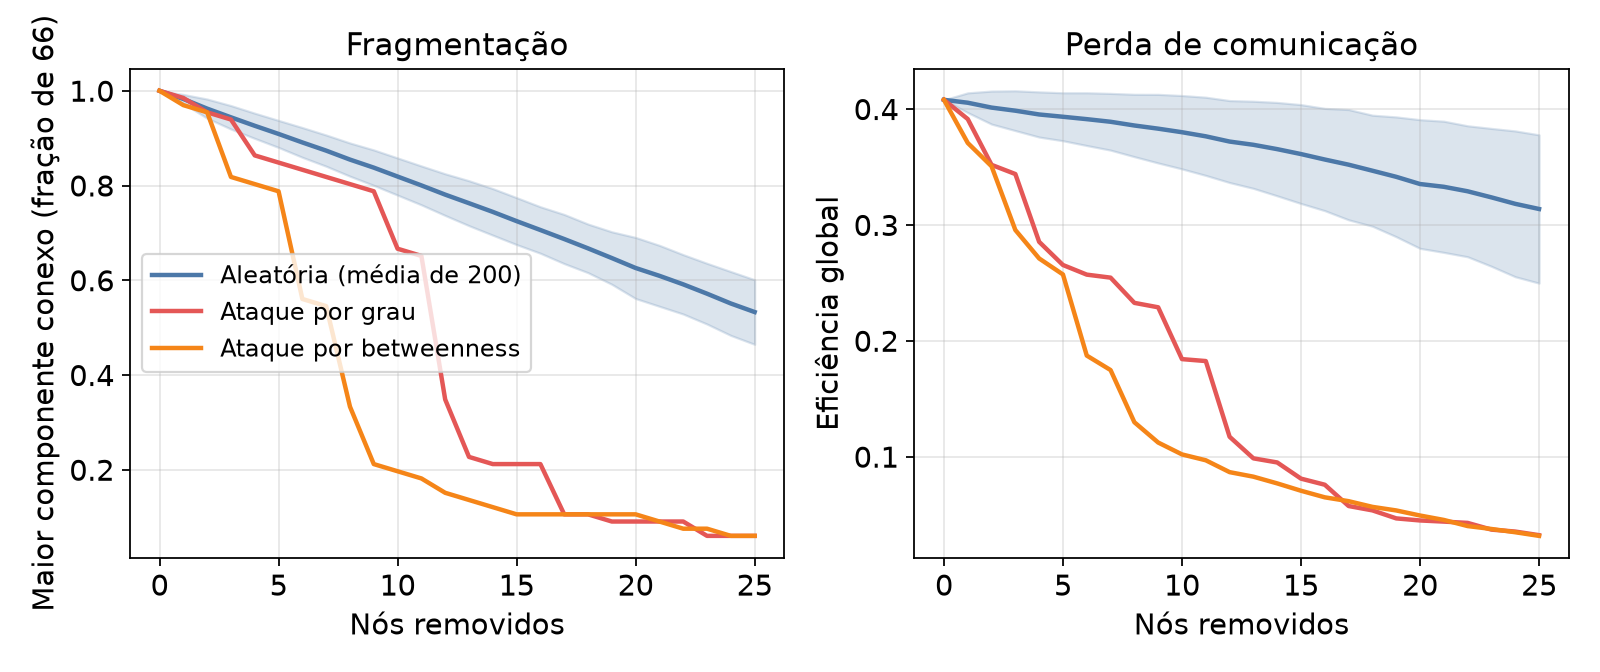
\includegraphics[width=\textwidth]{fig_robustez.png}
  \caption{Remoção de nós: ao acaso (média de 200 sorteios, com desvio padrão), por ataque ao grau e por ataque à betweenness.}
  \label{fig:robustez}
  \fonte{Elaborada pelos autores (Python, \textit{networkx}).}
\end{figure}

Cinco proteínas são pontos de articulação: \textbf{HTT, PPARGC1A, SLC1A2}, KCNJ10 e SLC6A11 (losangos na Figura~\ref{fig:impactorede}). A remoção individual que mais reduz a eficiência global é a do SLC1A2 (11,5\%), seguida de PPARGC1A (11,0\%) e HTT (9,1\%). O TP53, apesar do maior grau, reduz a eficiência em apenas 4,1\%, pois seus vizinhos continuam conectados por outros caminhos.

\begin{figure}[H]
  \centering
  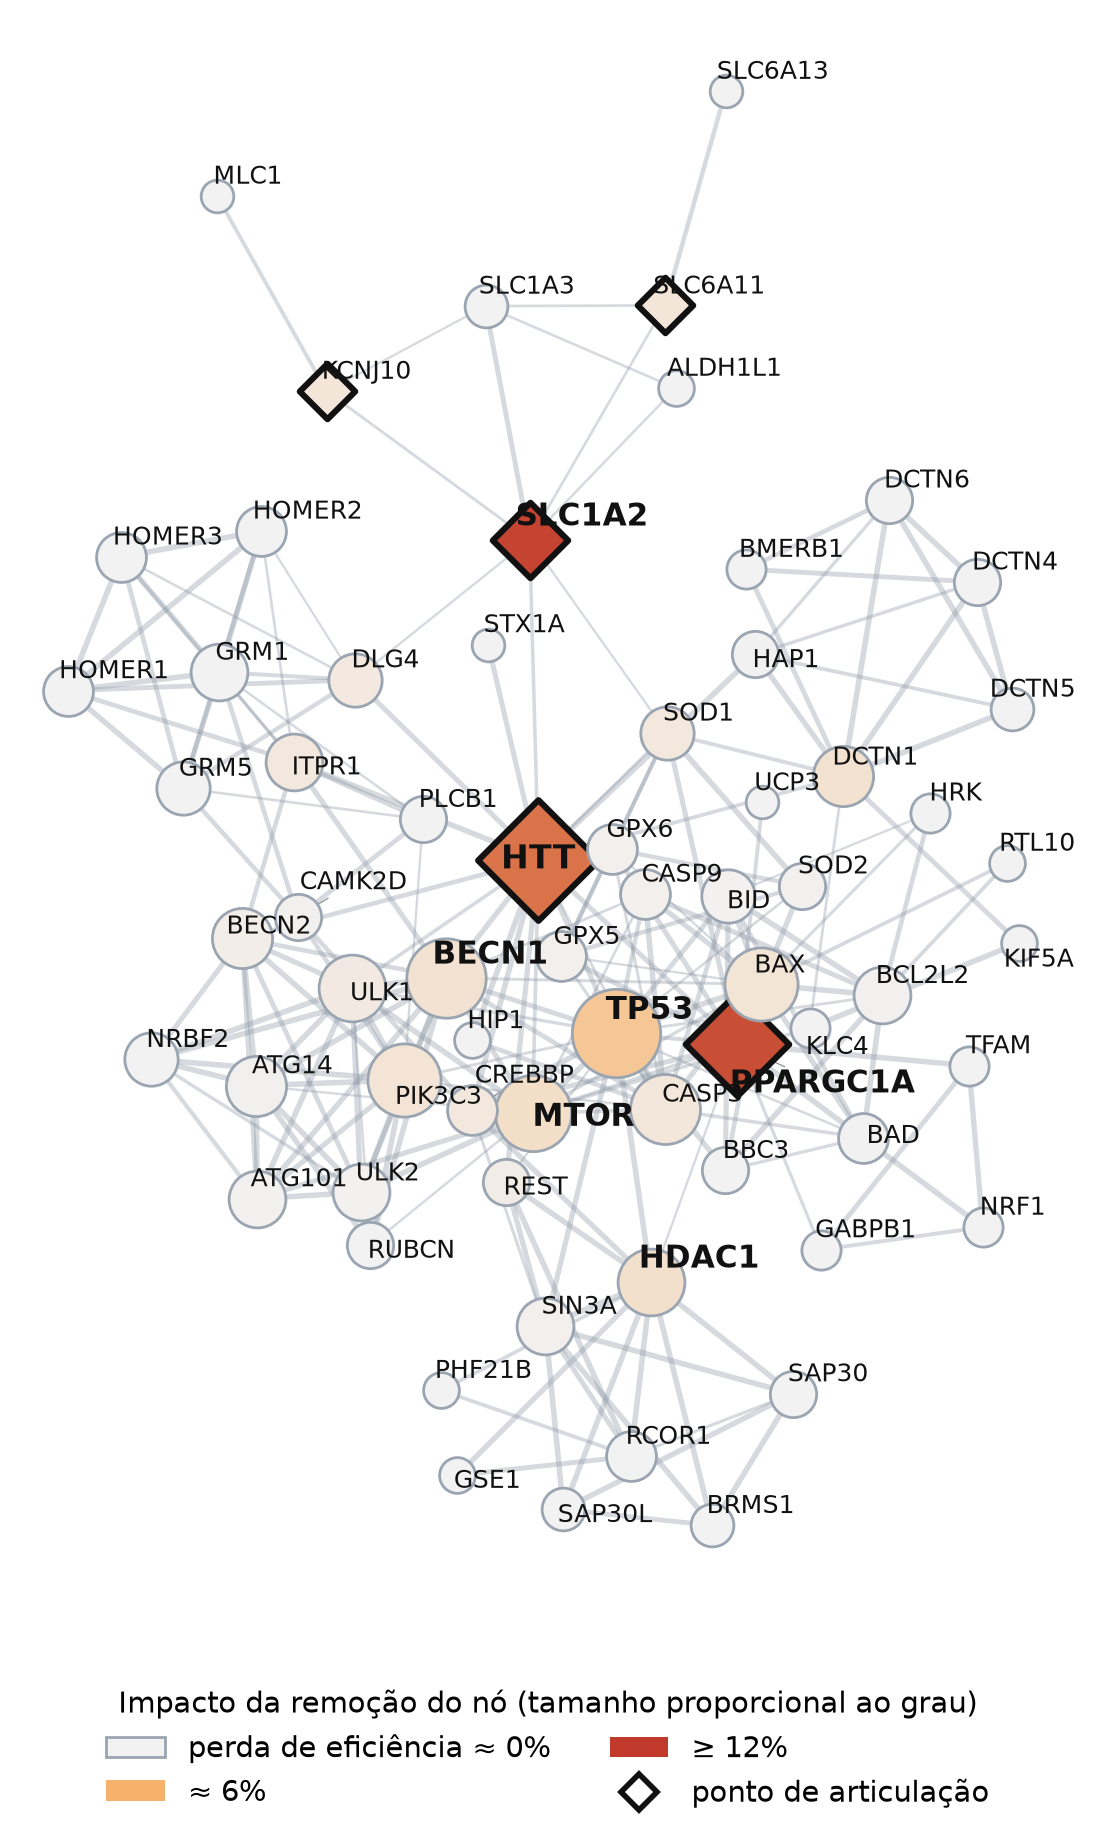
\includegraphics[width=\textwidth,height=0.78\textheight,keepaspectratio]{rede_impacto.png}
  \caption{Impacto da remoção de cada nó. A cor indica a perda de eficiência global e os losangos, os pontos de articulação.}
  \label{fig:impactorede}
  \fonte{Elaborada pelos autores, com layout do Cytoscape 3.10.5.}
\end{figure}

\subsection{Cascata de falha}

O resultado da cascata depende fortemente do limiar $\varphi$ (Figura~\ref{fig:cascata}). Para $\varphi = 0{,}2$, em média 19,9 nós falham, e 16 sementes derrubam mais da metade da rede (a partir do HTT, falham todos os 66 nós). Para $\varphi = 0{,}3$, a média cai para 3,0 e só a semente BAX derruba a rede inteira. Para $\varphi \geq 0{,}4$, a falha de um nó quase não se propaga (média de 1,4). A rede passa de estável para frágil em uma faixa estreita de limiar, e por isso o limiar precisa ser declarado como suposição.

\begin{figure}[H]
  \centering
  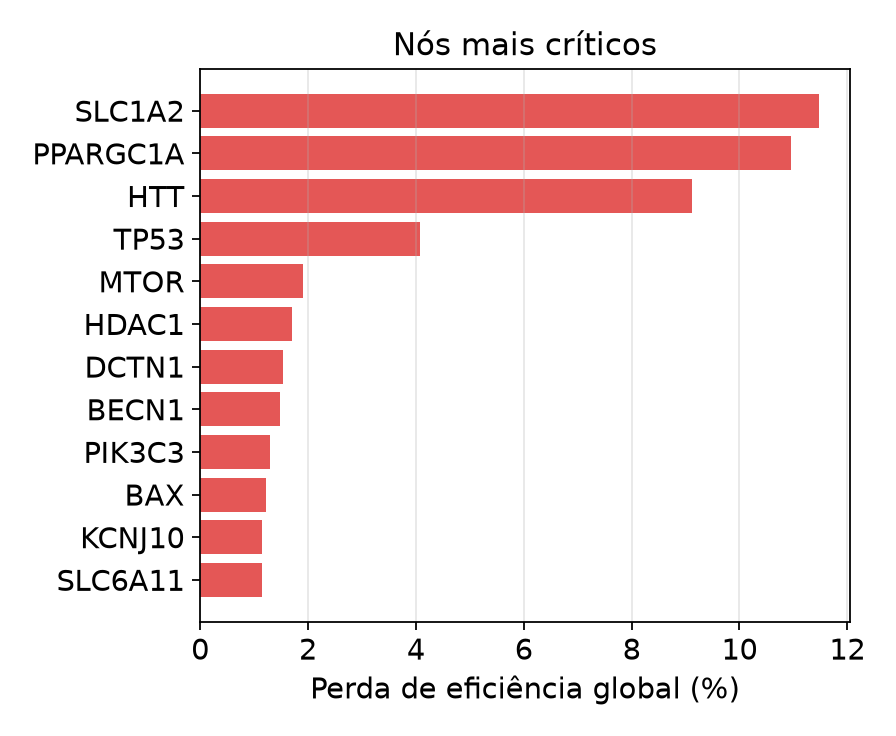
\includegraphics[width=0.48\textwidth]{fig_impacto_nos.png}\hfill
  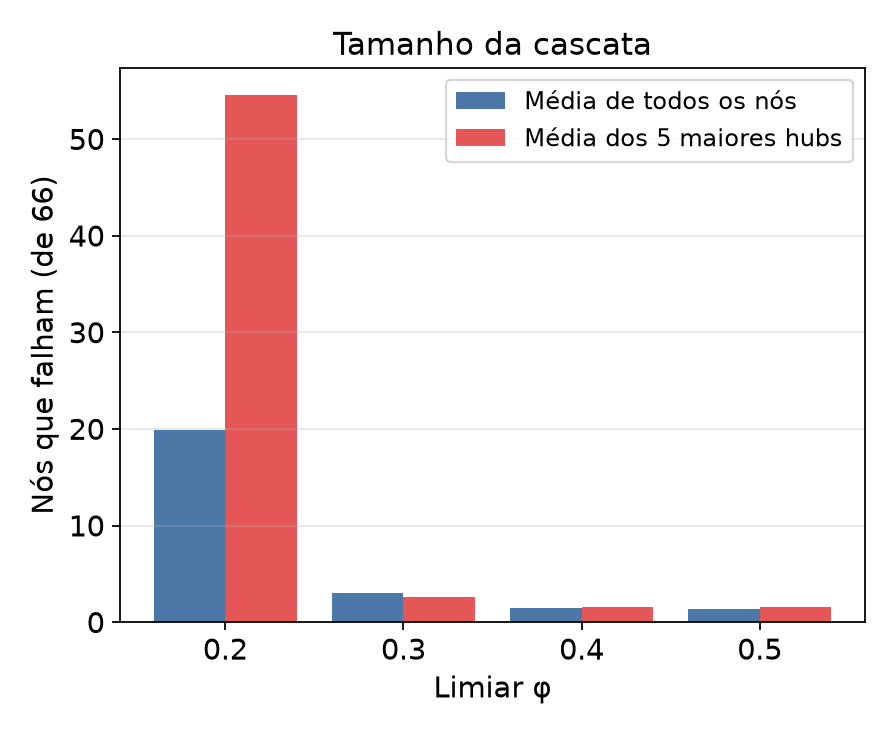
\includegraphics[width=0.48\textwidth]{fig_cascata.png}
  \caption{Esquerda: perda de eficiência global ao remover cada nó (12 maiores). Direita: tamanho médio da cascata por limiar $\varphi$.}
  \label{fig:cascata}
  \fonte{Elaborada pelos autores.}
\end{figure}

\subsection{Estratégia de proteção}

No regime frágil ($\varphi = 0{,}2$), em que a cascata média é de 19,9 nós, proteger os 5 nós de maior grau (TP53, HTT, BECN1, MTOR e PPARGC1A) reduz a cascata média para 6,8 nós (queda de 66\%), contra 16,5 nós (queda de 17\%) ao proteger 5 proteínas sorteadas (Figura~\ref{fig:protecao}). Proteger apenas o HDAC1 já reduz a cascata para 14,5 nós (27\%). A escolha gulosa foi a melhor até 3 proteínas, mas não superou a escolha por grau com 5, pois decide um passo de cada vez. Para $\varphi = 0{,}3$ o efeito em números absolutos é pequeno, porque a cascata já é curta: a média cai de 3,0 para 2,2 nós com 5 proteínas protegidas por grau e para 1,4 pela escolha gulosa.

\begin{figure}[H]
  \centering
  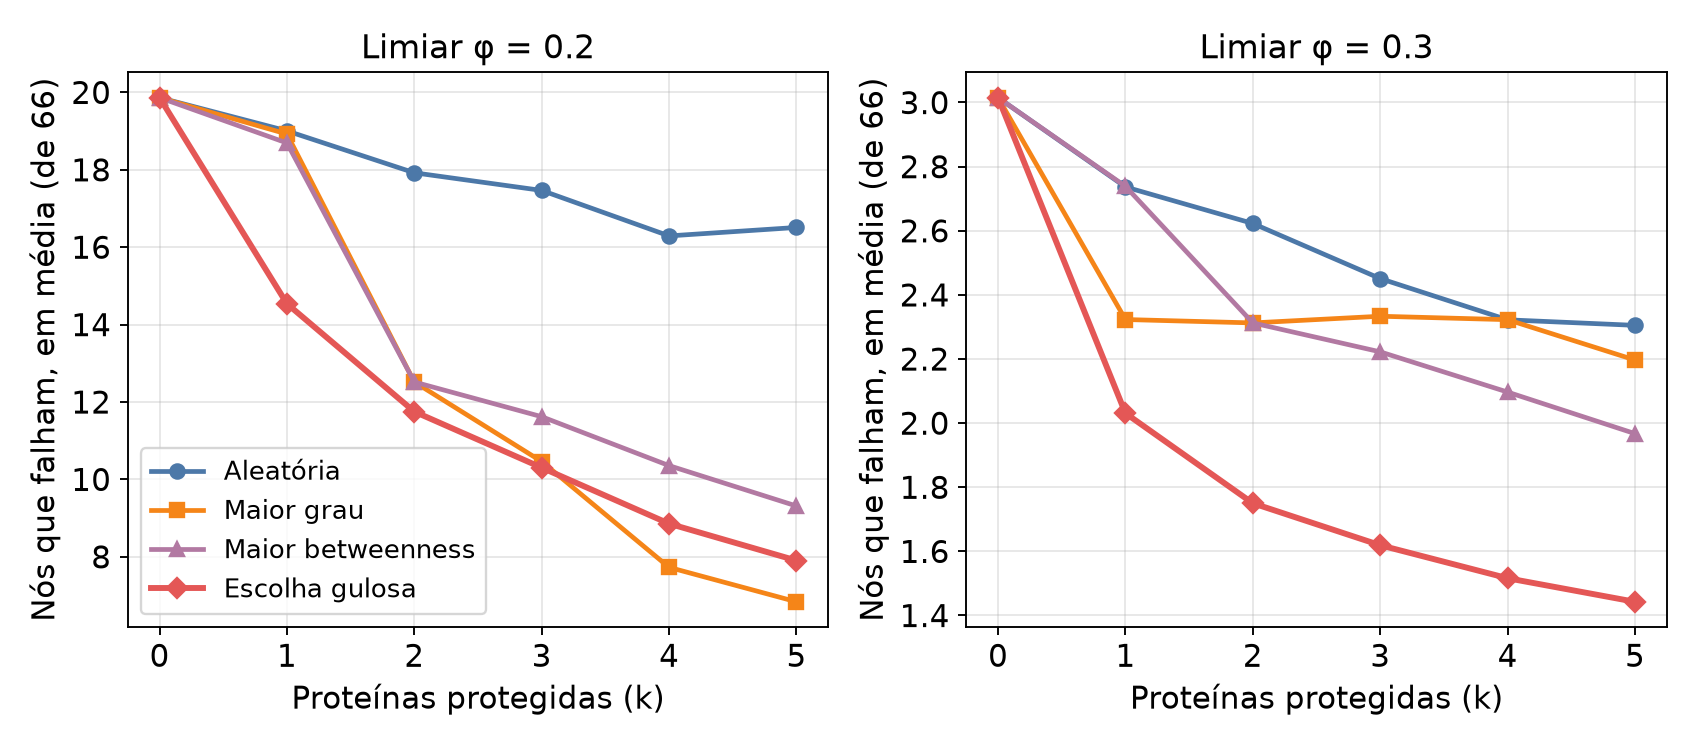
\includegraphics[width=\textwidth]{fig_protecao.png}
  \caption{Tamanho médio da cascata ao proteger de 0 a 5 proteínas, escolhidas de quatro formas, para dois limiares.}
  \label{fig:protecao}
  \fonte{Elaborada pelos autores (Python, \textit{networkx}).}
\end{figure}

% ===================== 4. DISCUSSÃO =====================
\section{Discussão}

\textbf{Interpretação.} A rede do HTT é robusta a falhas aleatórias e frágil a ataques a poucos nós centrais. O HTT é ao mesmo tempo o nó de maior betweenness e um ponto de articulação, o que combina com seu papel de ligar processos celulares distintos. Também ligam módulos inteiros ao resto o PPARGC1A (mitocôndria e estresse oxidativo), cuja repressão pelo HTT mutado já foi descrita \cite{cui2006}, e o SLC1A2 (captação de glutamato pelos astrócitos), cuja alteração na DH é discutida na literatura \cite{khakh2017}. Esses resultados descrevem a estrutura da rede e não a função: a rede é estática, sem direção nem sinal, e remover o HTT testa a dependência da rede, mas não reproduz a ação tóxica da mutação.

\textbf{Alvos candidatos.} Os nós que aparecem tanto na fragmentação quanto na cascata são PPARGC1A, SLC1A2 e HTT (Tabela~\ref{tab:alvos}). Isso sugere duas frentes de investigação: o metabolismo mitocondrial e a captação de glutamato pelos astrócitos. A simulação de proteção reforça essa leitura: manter funcionais os hubs, entre eles o PPARGC1A e o HTT, contém a maior parte da cascata (Figura~\ref{fig:protecao}). São hipóteses geradas pela topologia, e não conclusões clínicas, e precisam ser confrontadas com a literatura experimental.

\begin{table}[H]
  \centering
  \caption{Nós candidatos a alvo de investigação, com seu papel fisiológico e o que a rede indica.}
  \label{tab:alvos}
  \footnotesize
  \begin{tabular}{p{1.8cm}p{4.6cm}p{5.6cm}}
    \toprule
    Proteína & Papel fisiológico & Evidência na rede \\
    \midrule
    HTT & Proteína de andaime ligada ao transporte de vesículas, à transcrição e à sobrevivência neuronal & Maior betweenness (0,399); ponto de articulação; liga os 7 módulos \\
    PPARGC1A & Coativador que regula a biogênese mitocondrial e o metabolismo energético do neurônio & Ponto de articulação; 2º maior impacto na eficiência (11,0\%) \\
    SLC1A2 & Transportador (EAAT2) que retira o glutamato da fenda sináptica, nos astrócitos, e limita a entrada excessiva de cálcio & Ponto de articulação; maior impacto na eficiência (11,5\%) com apenas 7 conexões \\
    TP53 & Regulador central da apoptose & Maior grau (18), mas baixo impacto na remoção (4,1\%) \\
    MTOR, BECN1 & Controle da autofagia, que degrada proteínas agregadas & Hubs do módulo mais conectado (grau 14 e 15) \\
    \bottomrule
  \end{tabular}
\end{table}

% ===================== 5. CONCLUSÃO =====================
\section{Conclusão}

A rede PPI do HTT (66 proteínas, 207 interações) é conexa, agrupada e organizada nos módulos funcionais da doença ($Q = 0{,}60$). O TP53 tem o maior grau, mas HTT, SLC1A2 e PPARGC1A são as pontes entre os módulos, e sua remoção fragmenta a rede. Proteger os cinco principais hubs reduz a cascata simulada em 66\%, contra 17\% ao proteger proteínas sorteadas. A rede também tem a propriedade de mundo pequeno ($\sigma = 5{,}6$). Mitocôndria e astrócitos são as frentes de investigação sugeridas. São hipóteses a testar, e não conclusões clínicas.

\newpage
\addcontentsline{toc}{section}{Referências}
\begin{thebibliography}{99}

\bibitem[ALBERT; JEONG; BARABÁSI, 2000]{albert2000}
ALBERT, R.; JEONG, H.; BARABÁSI, A.-L. Error and attack tolerance of complex networks. \textbf{Nature}, v. 406, p. 378--382, 2000.

\bibitem[BARABÁSI; OLTVAI, 2004]{barabasi2004}
BARABÁSI, A.-L.; OLTVAI, Z. N. Network biology: understanding the cell's functional organization. \textbf{Nature Reviews Genetics}, v. 5, p. 101--113, 2004.

\bibitem[BLONDEL et al., 2008]{blondel2008}
BLONDEL, V. D. et al. Fast unfolding of communities in large networks. \textbf{Journal of Statistical Mechanics}, P10008, 2008.

\bibitem[BULDYREV et al., 2010]{buldyrev2010}
BULDYREV, S. V. et al. Catastrophic cascade of failures in interdependent networks. \textbf{Nature}, v. 464, p. 1025--1028, 2010.

\bibitem[CARON; WRIGHT; HAYDEN, 2020]{genereviews}
CARON, N. S.; WRIGHT, G. E. B.; HAYDEN, M. R. Huntington disease. In: ADAM, M. P. et al. (ed.). \textbf{GeneReviews}. Seattle: University of Washington, 1998--2020. Disponível em: \url{https://www.ncbi.nlm.nih.gov/books/NBK1305/}. [atualizado em 11 jun. 2020].

\bibitem[CUI et al., 2006]{cui2006}
CUI, L. et al. Transcriptional repression of PGC-1$\alpha$ by mutant huntingtin leads to mitochondrial dysfunction and neurodegeneration. \textbf{Cell}, v. 127, p. 59--69, 2006.

\bibitem[HDCRG, 1993]{htt1993}
THE HUNTINGTON'S DISEASE COLLABORATIVE RESEARCH GROUP. A novel gene containing a trinucleotide repeat that is expanded and unstable on Huntington's disease chromosomes. \textbf{Cell}, v. 72, p. 971--983, 1993.

\bibitem[KANEHISA; GOTO, 2000]{kegg2000}
KANEHISA, M.; GOTO, S. KEGG: Kyoto Encyclopedia of Genes and Genomes. \textbf{Nucleic Acids Research}, v. 28, n. 1, p. 27--30, 2000. 

\bibitem[KEGG, 2020]{keggpath}
KANEHISA LABORATORIES. \textbf{KEGG PATHWAY: Huntington disease (hsa05016)}. Disponível em: \url{https://www.kegg.jp/entry/hsa05016}. Acesso em: 13--14 nov. 2026.

\bibitem[KHAKH et al., 2017]{khakh2017}
KHAKH, B. S. et al. Unravelling and exploiting astrocyte dysfunction in Huntington's disease. \textbf{Trends in Neurosciences}, v. 40, p. 422--437, 2017.

\bibitem[MEDINA et al., 2022]{medina2022}
MEDINA, A. et al. Prevalence and incidence of Huntington's disease: an updated systematic review and meta-analysis. \textbf{Movement Disorders}, v. 37, n. 12, p. 2327--2335, 2022. 

\bibitem[NEWMAN, 2006]{newman2006}
NEWMAN, M. E. J. Modularity and community structure in networks. \textbf{Proceedings of the National Academy of Sciences}, v. 103, n. 23, p. 8577--8582, 2006.

\bibitem[SHANNON et al., 2003]{shannon2003}
SHANNON, P. et al. Cytoscape: a software environment for integrated models of biomolecular interaction networks. \textbf{Genome Research}, v. 13, p. 2498--2504, 2003.

\bibitem[STRING, 2023b]{stringsite}
STRING CONSORTIUM. \textbf{STRING: functional protein association networks}. Disponível em: \url{https://string-db.org}. Acesso em: 13--14 nov. 2026.

\bibitem[SZKLARCZYK et al., 2025]{string2025}
SZKLARCZYK, D. et al. The STRING database in 2025: protein networks with directionality of regulation. \textbf{Nucleic Acids Research}, v. 53, n. D1, p. D730--D737, 2025.

\end{thebibliography}

% ===================== APÊNDICE =====================
\newpage
\section*{Apêndice A: mapa da Doença de Huntington (KEGG)}

\begin{figure}[H]
  \centering
  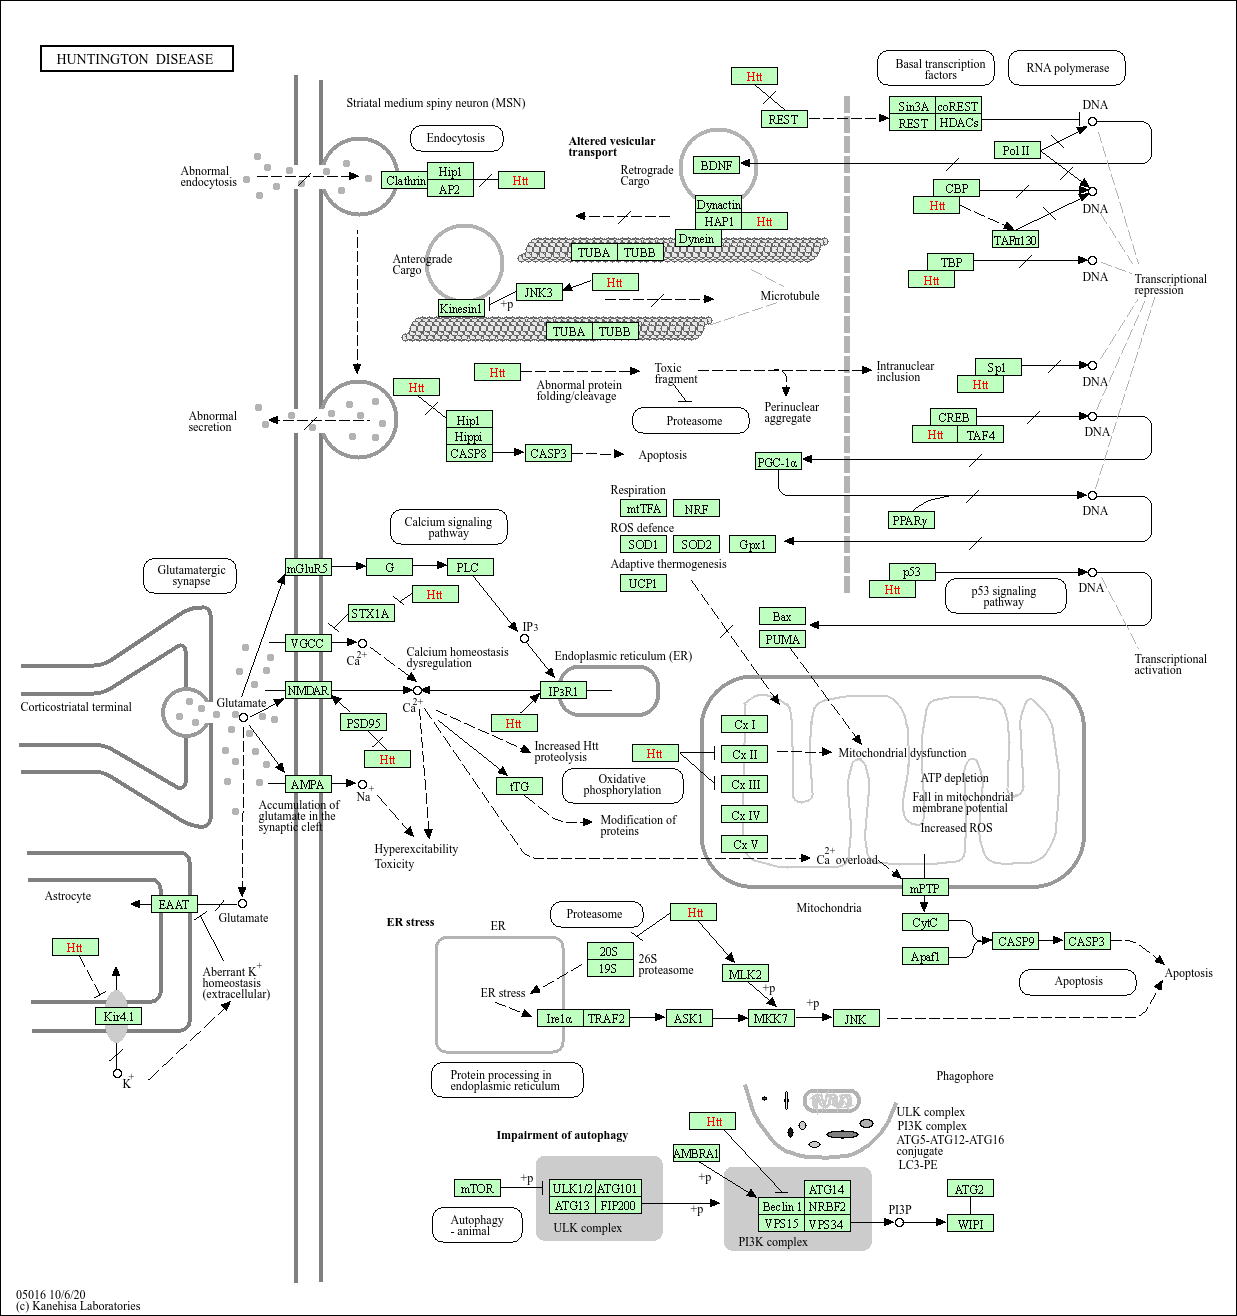
\includegraphics[width=0.97\textwidth]{kegg_huntington.png}
  \caption{Mapa da Doença de Huntington (hsa05016) no KEGG, usado para definir os sete grupos de proteínas da rede.}
  \fonte{KEGG PATHWAY, hsa05016, Kanehisa Laboratories \cite{keggpath}.}
\end{figure}

\end{document}
